\section{Experimentación Y Resultados}

  Los algoritmos previamente detallados tienen muchos puntos a testear. Veamos cada uno de estos en forma detallada y con los resultados intentemos responder a la pregunta original: ¿qué estrategia debo tomar para posicionar mi sitio en internet?

  \begin{itemize}
    \item{Convergencia de Page Rank}
    \item{Convergencia de Hits}
    \item{Comparación de tiempos}
  \end{itemize}


\subsection{Casos de prueba}
   A continuación se listarán los casos utilizados en las experimentaciones para mayor comprensión de los casos.

	\begin{itemize}
		\item MOVIES: Este caso incluye 5797 páginas
		\item ABORTION: Este caso incluye 2293 páginas
		\item GENETIC: Este caso incluye 3468 páginas
		\item STANFORD: Este caso incluye 281903 páginas
		\item GOOGLE: Este caso incluye 916428 páginas
	\end{itemize}  

\subsection{Convergencia de Page Rank} 

La convergencia de dicho algoritmo ocurrirá cuando la norma Manhattan de los vectores de la iteración anterior y la del actual sea cero(o a un valor relativamente cerca, esta cercanía estará dada por una tolerancia que para los casos presentados son cero). Es ahí cuando tendremos la respuesta final.\\
Para evaluar el comportamiento de la norma manhattan variaremos la probabilidad del navegante aleatorio, el cual de ahora en más lo denotaremos como el parámetro \textbf{c}.\\
A continuación se muestran los resultados de como evoluciona la norma a lo largo de las iteraciones y como varía la misma con distintos c, y que luego discutiremos más adelante.
Cabe aclarar que expresamos los valores de la norma en escala logarítmica para una mejor visualización y para que se obtenga un mejor entendimiento de como disminuye de a varias magnitudes en cada iteración.


% \begin{figure}
% \begin{center}
       % 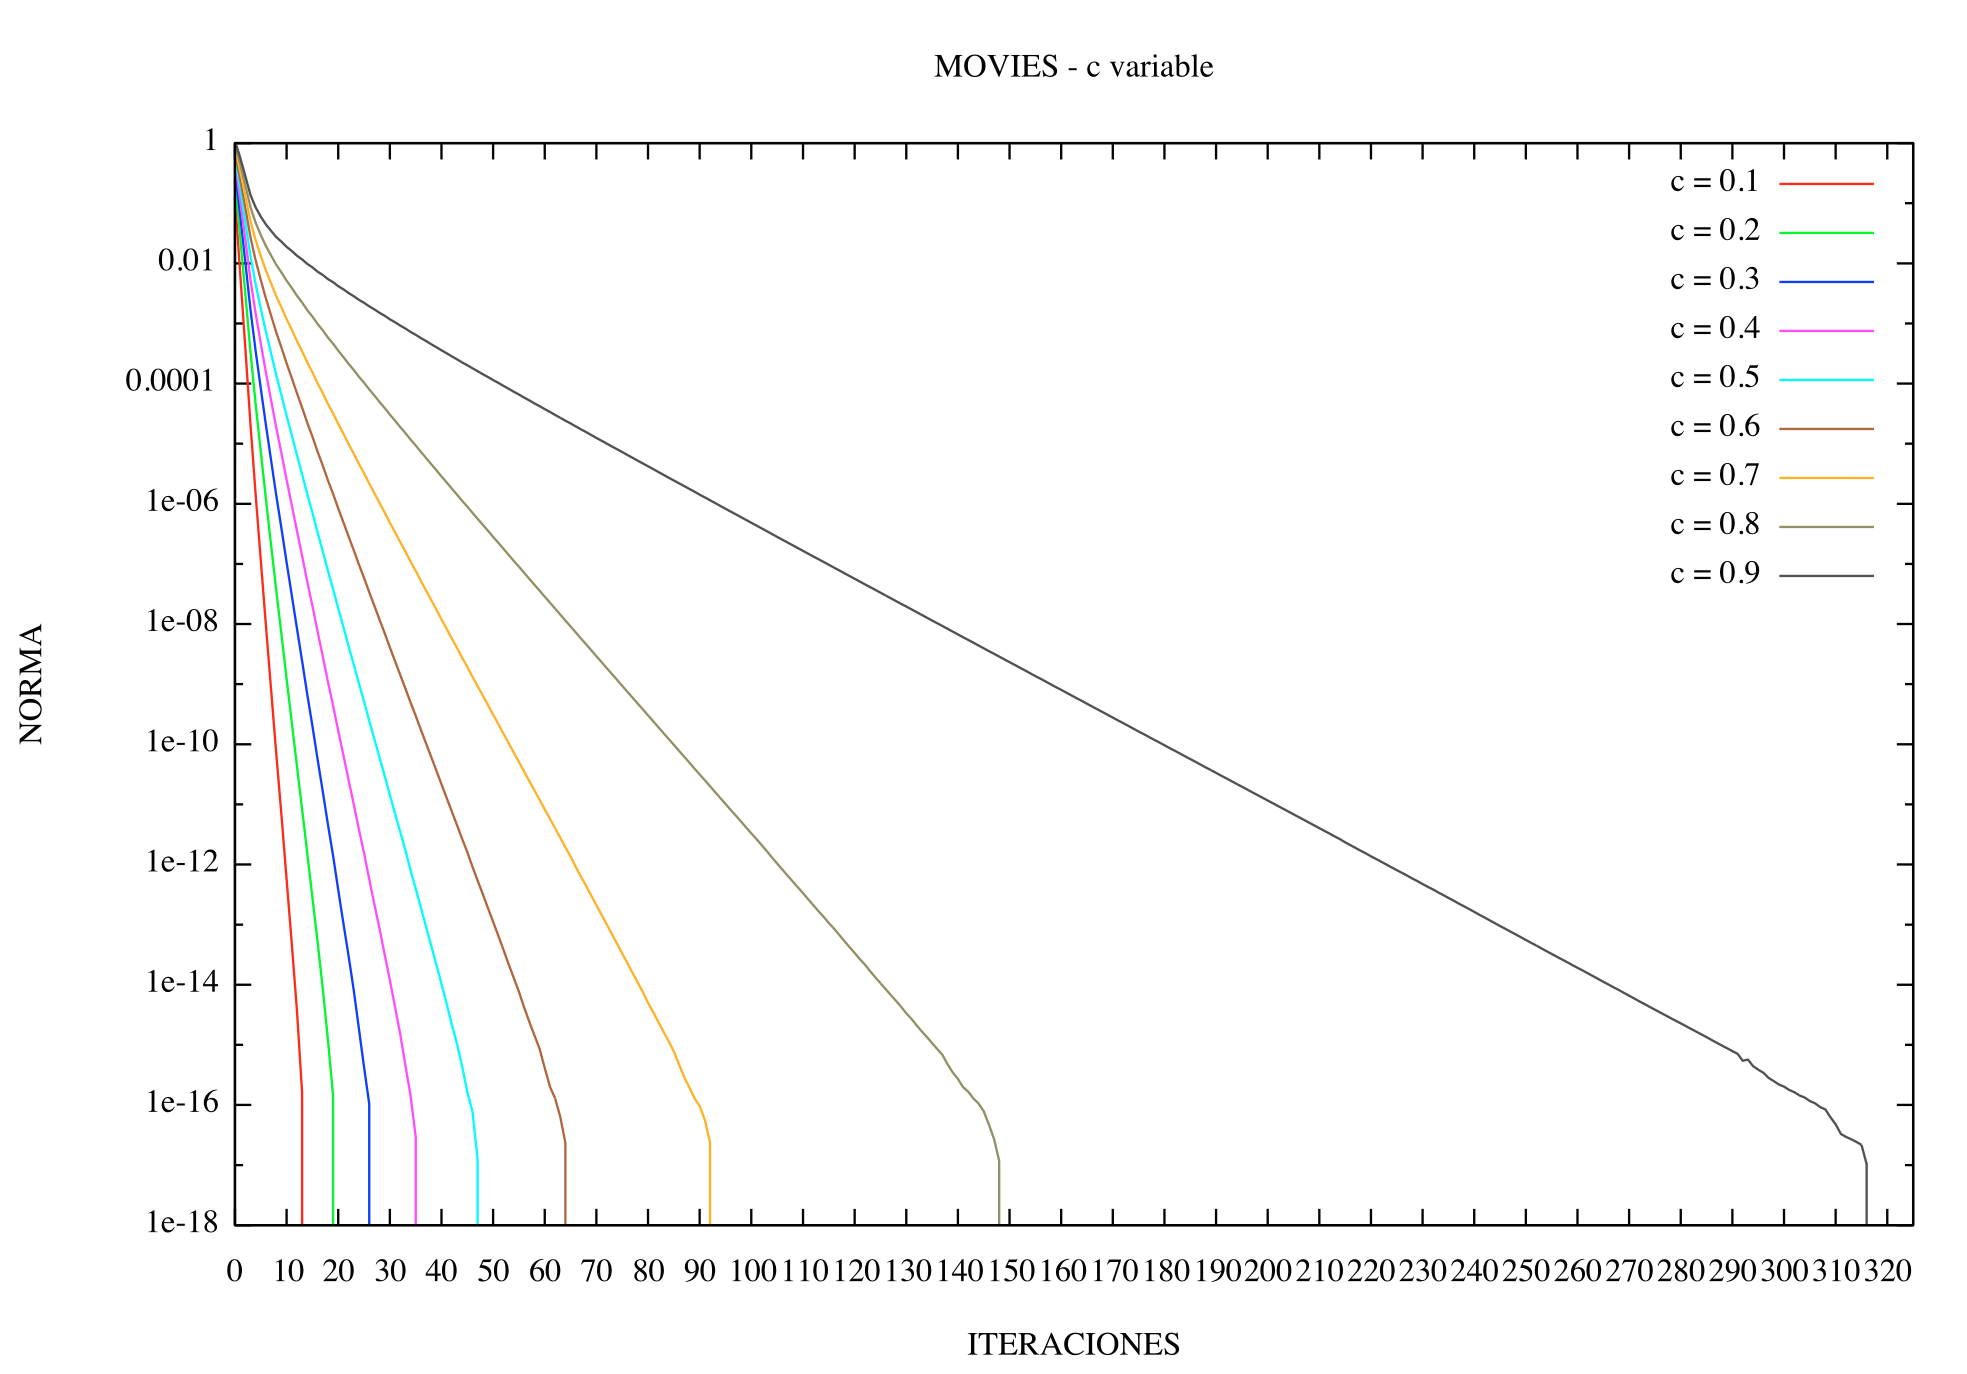
\includegraphics[scale=0.5]{imagenes/pagerank_movies_norma.png}
        % 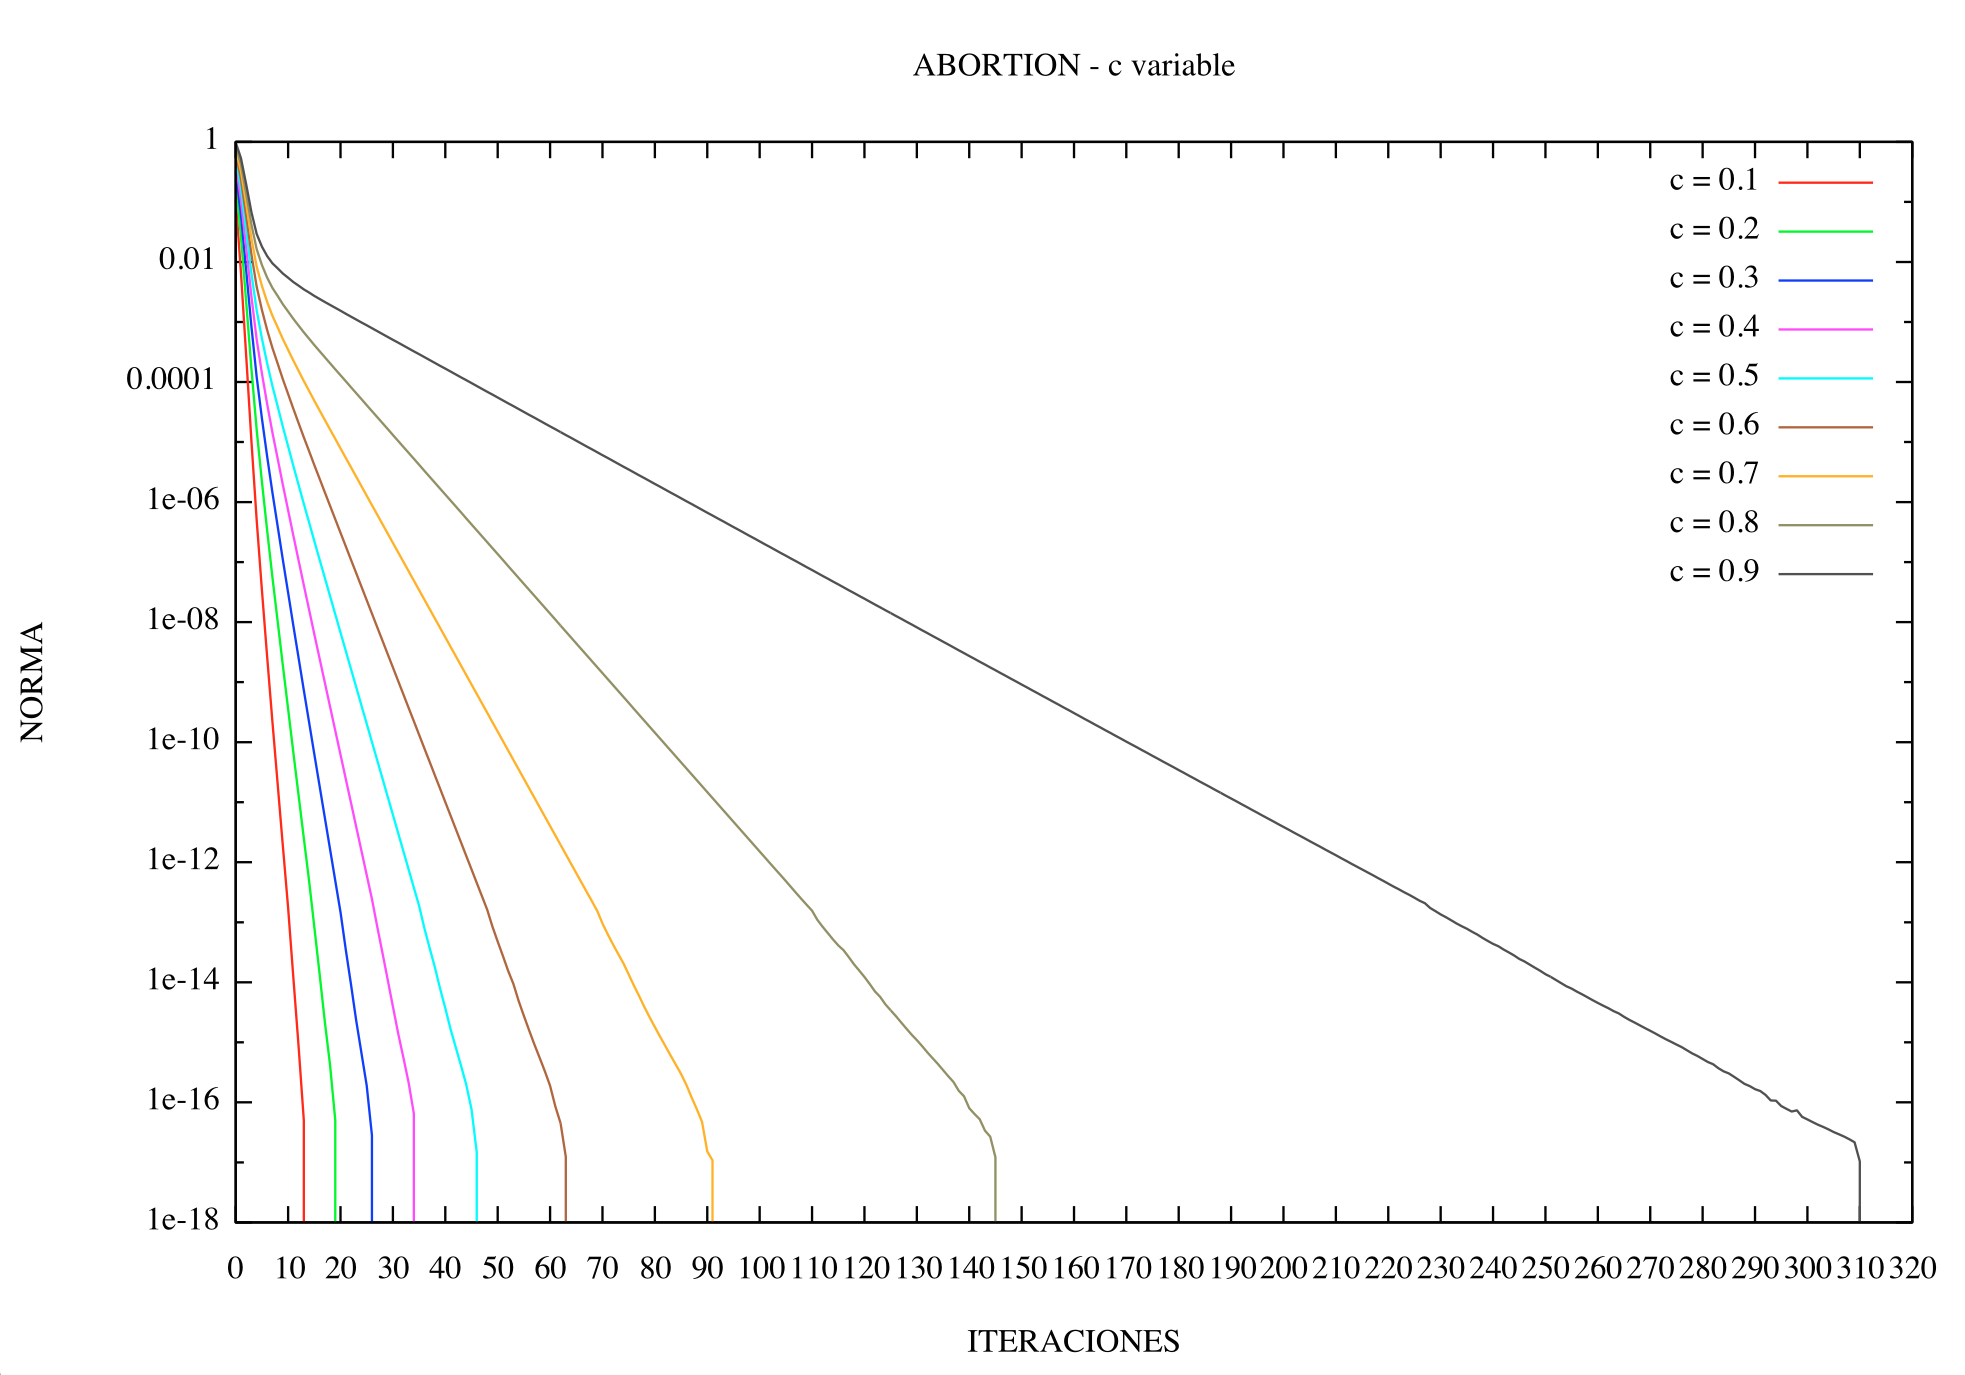
\includegraphics[scale=0.5]{imagenes/pagerank_abortion_norma.png}
       % \end{center}
% \end{figure}

\begin{figure}[!htb]
\begin{center}
    % 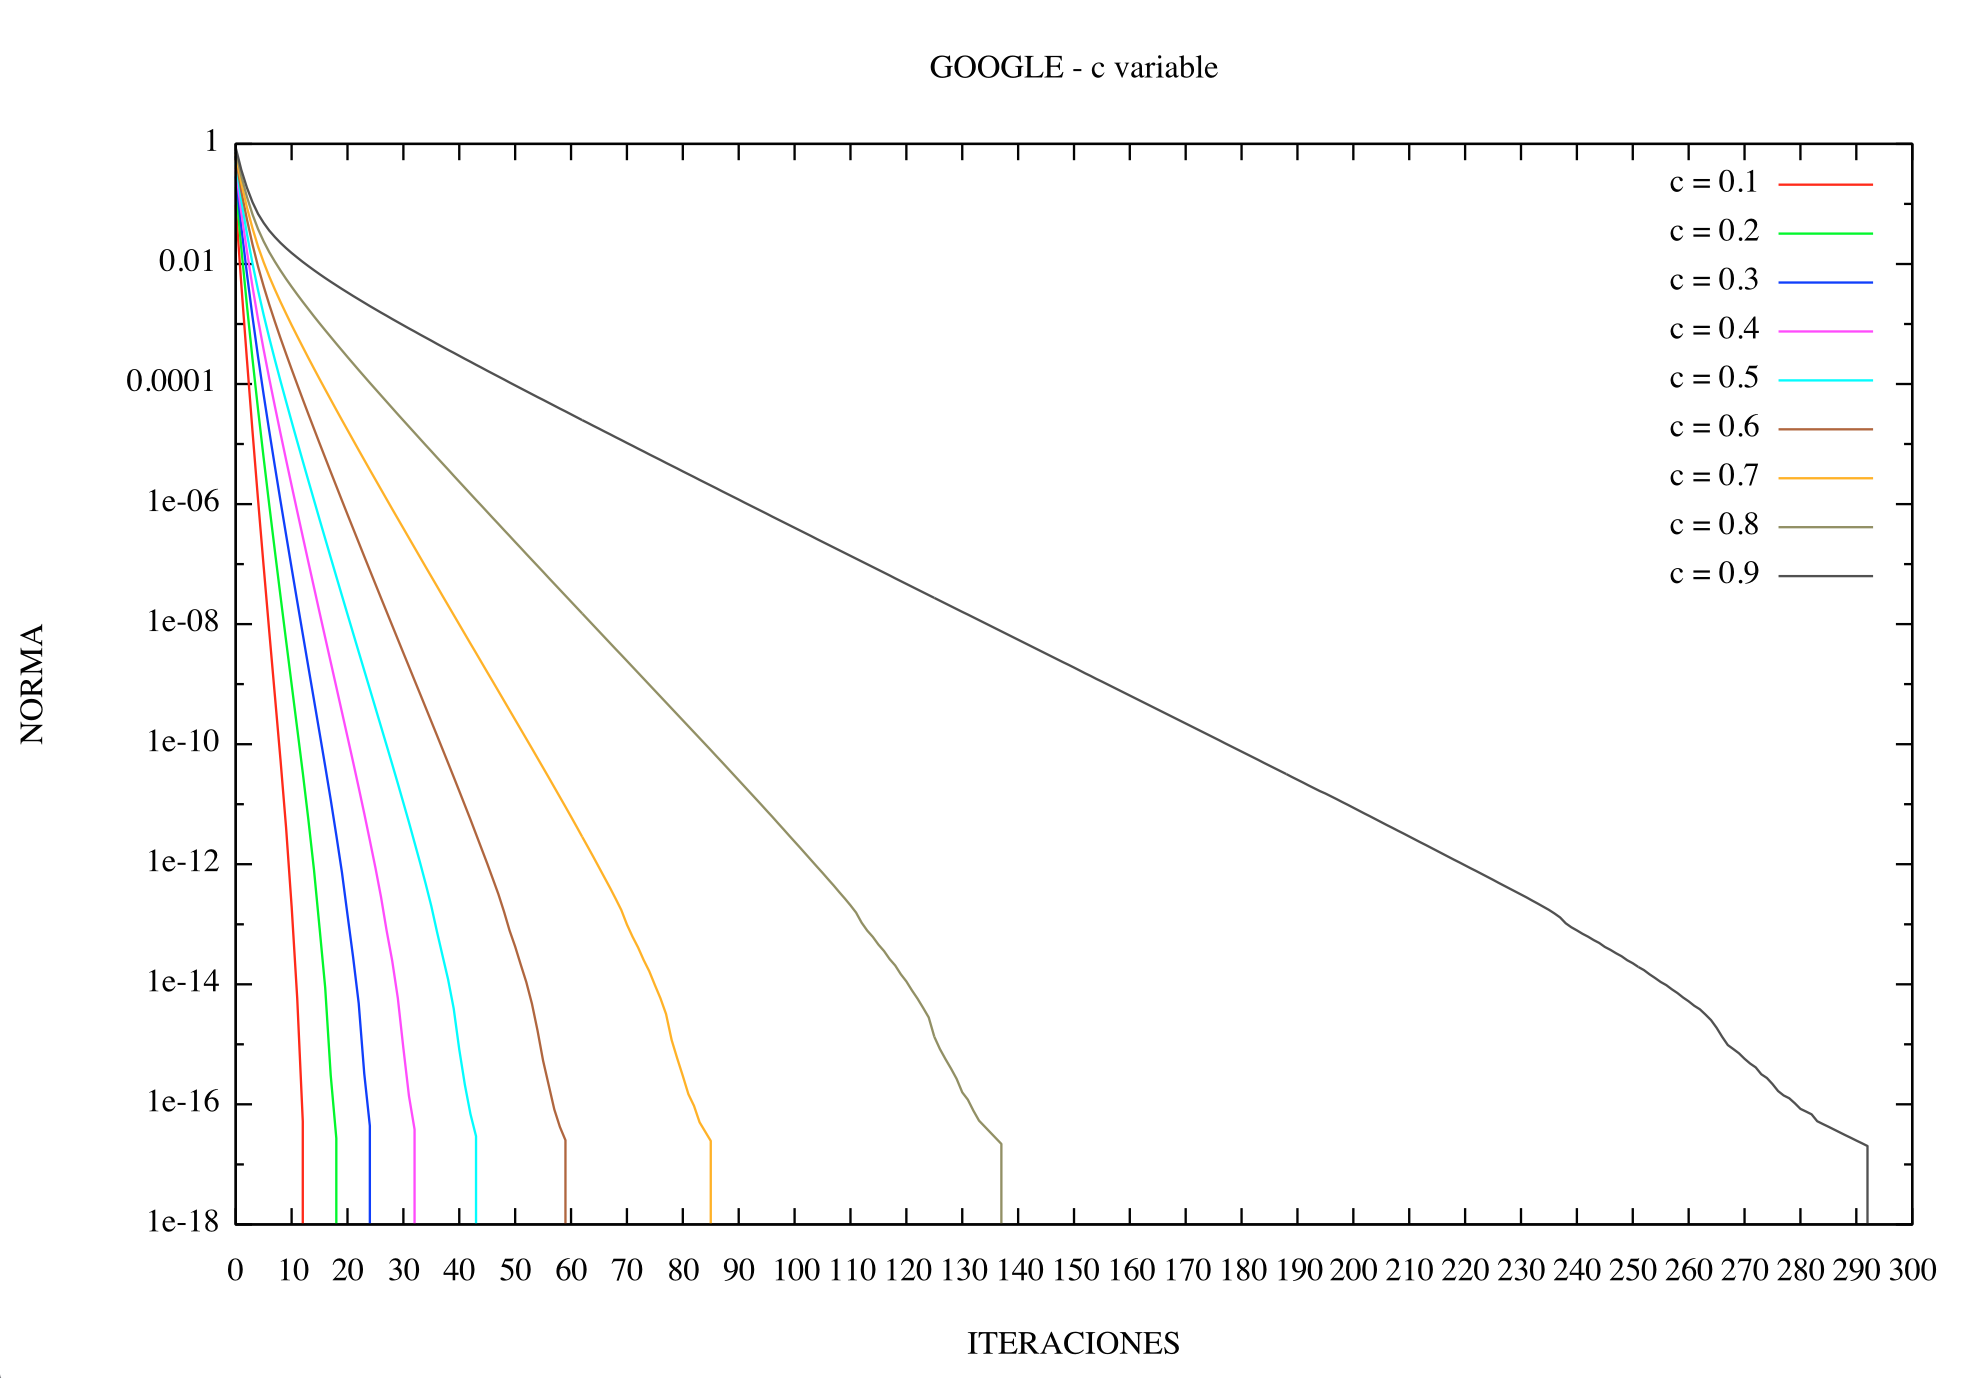
\includegraphics[scale=0.5]{imagenes/pagerank_google_norma.png}
  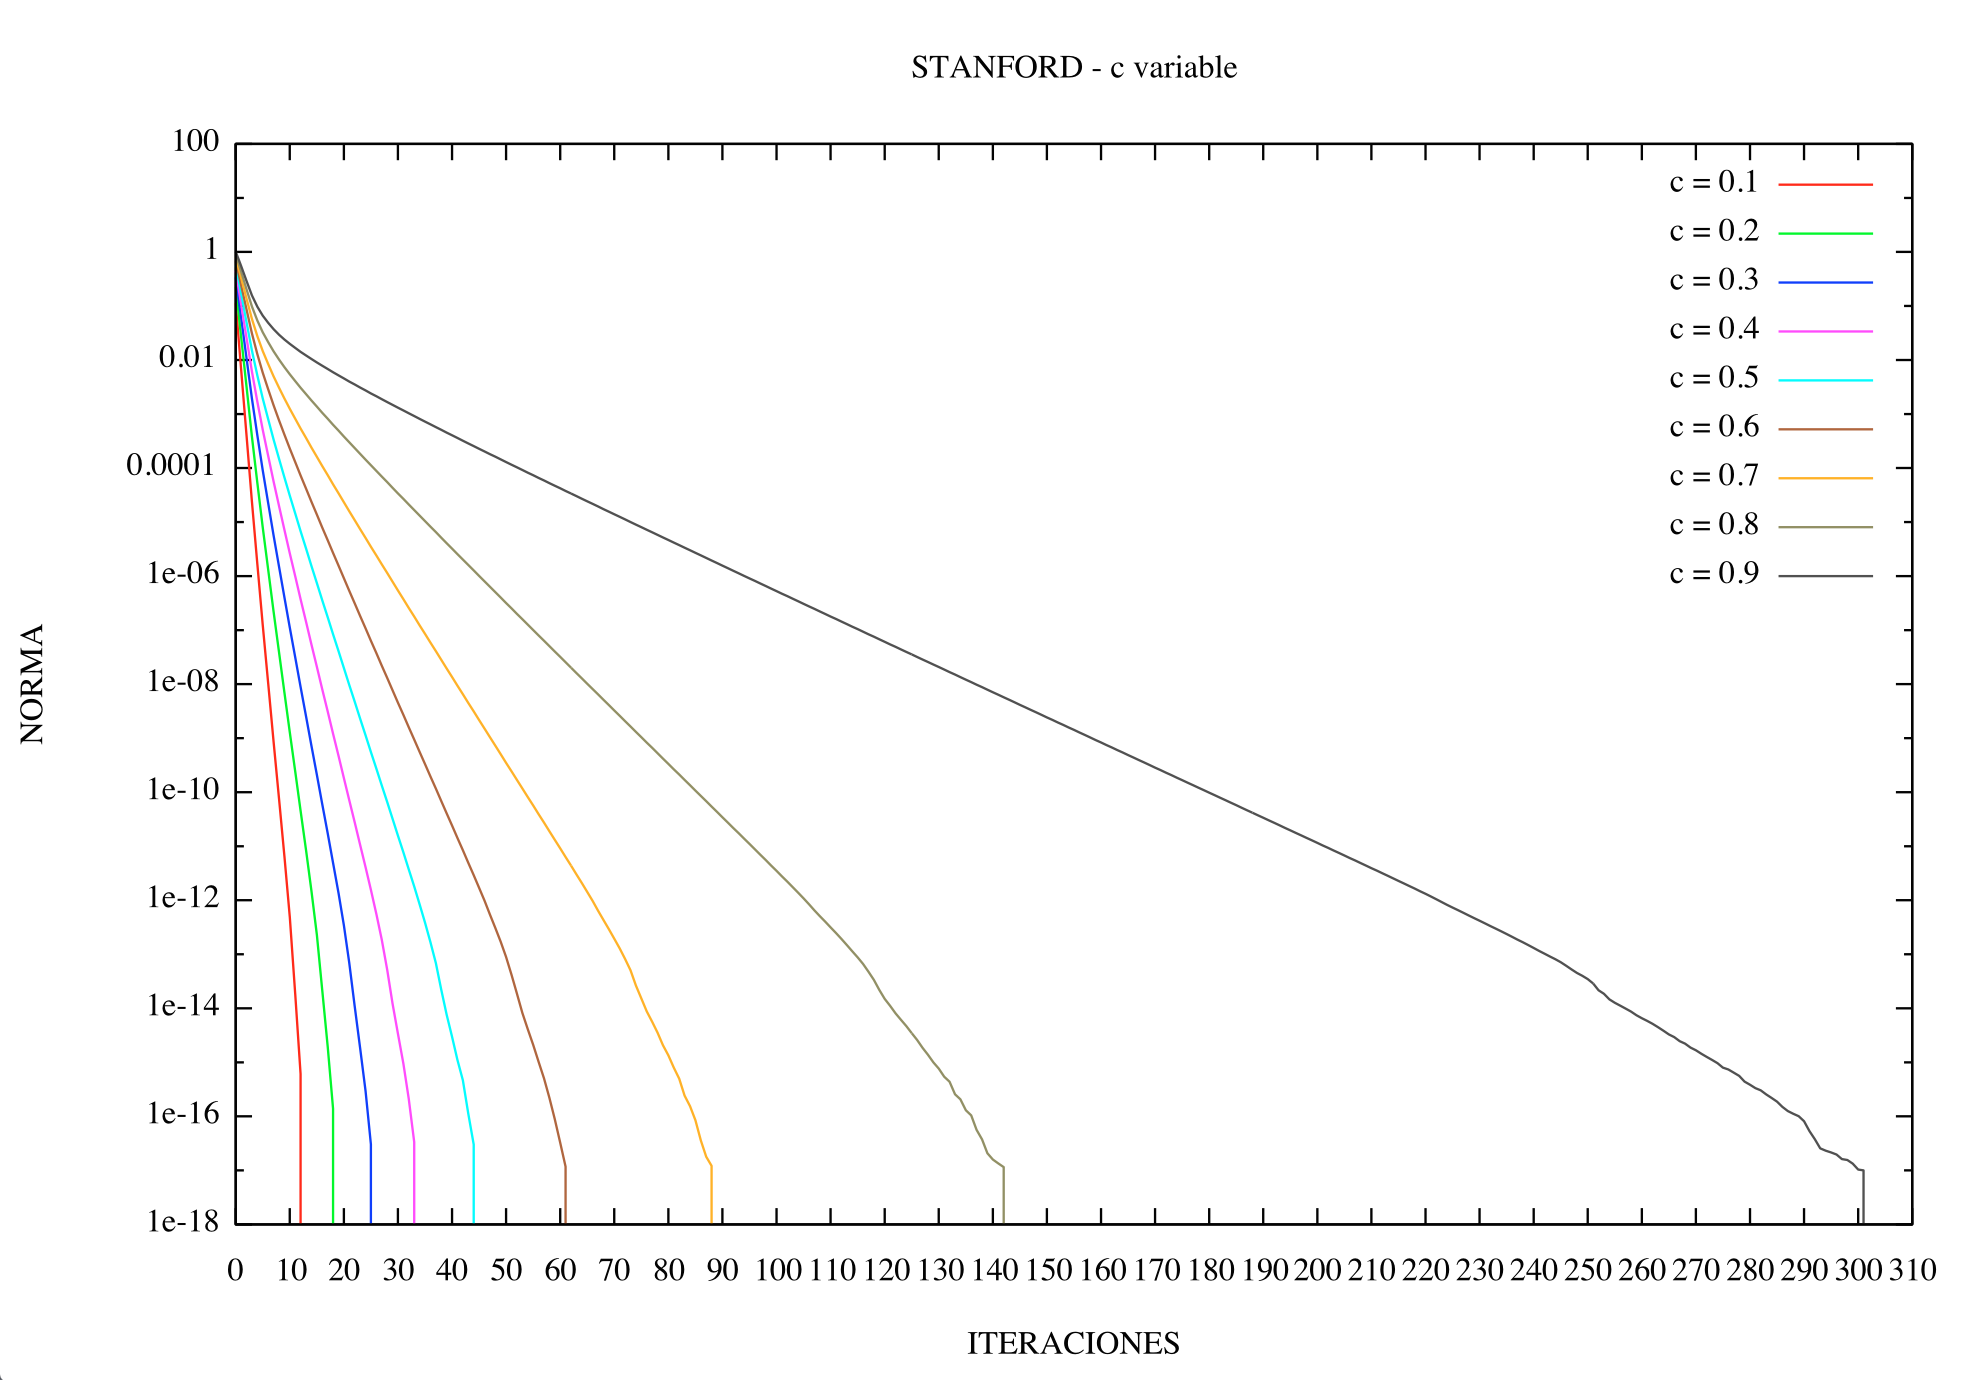
\includegraphics[scale=0.5]{imagenes/pagerank_stanford_norma.png}
    \end{center}
\end{figure}

De los casos de prueba presentados, agregamos solo este ya que el resto de los resultados eran iguales. Claramente notamos que la convergencia se retrasa más a medida que se agranda el c. 

\clearpage

\subsection {Convergencia de HITS}

La convergencia de dicho algoritmo ocurrirá cuando la norma Manhattan de los vectores x e y (que contienen el puntaje de los sitios de autoridad y los de hubs respectivamente) comparados con los de la iteración anterior 
sea cero para alguno de los dos(o a un valor relativamente cerca). Es ahí cuando tendremos la respuesta final.\\
Al igual que el algoritmo anterior utilizamos una tolerancia igual a cero.

A continuación se muestran los resultados para cuatro instancias distintas, 3 medianas y una grande, de como evoluciona la norma a lo largo de las iteraciones en ambos vectores :

\begin{figure}[!htb]
% \begin{center}
\begin{subfigure}{.5\textwidth}
       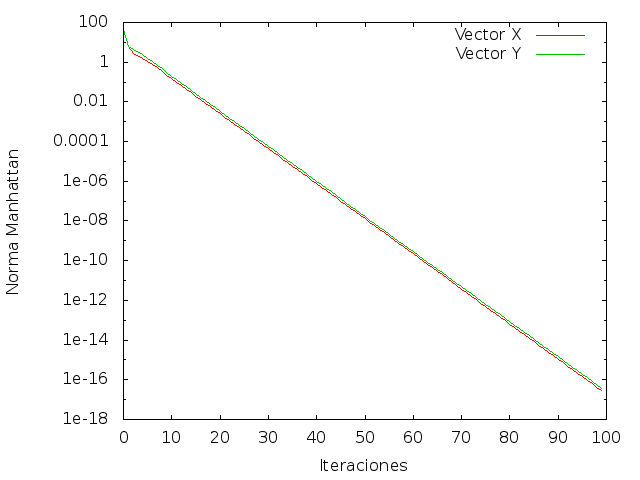
\includegraphics[scale=0.4]{imagenes/hits-abortion-expanded.png}
       \caption{Abortion expanded }
\end{subfigure}
  % \end{center}
% \end{figure}
% \begin{figure}
% \begin{center}
\begin{subfigure}{.5\textwidth}
        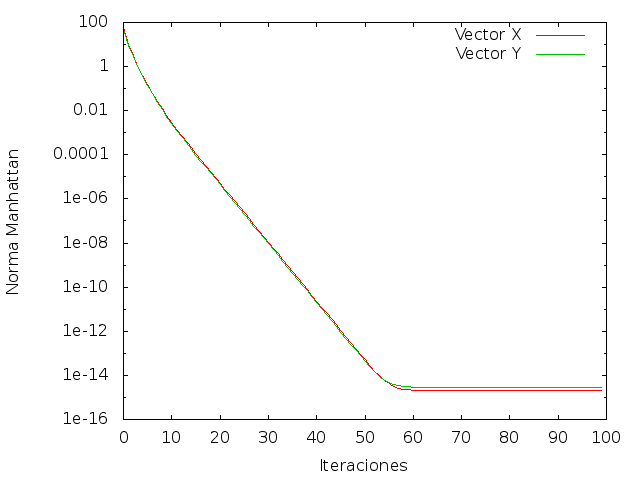
\includegraphics[scale=0.4]{imagenes/hits-genetic-expanded.png}
       \caption{Genetic expanded }
\end{subfigure}
       % \end{center}
% \end{figure}

% \begin{figure}[!htb]
% \begin{center}
\begin{subfigure}{.5\textwidth}
    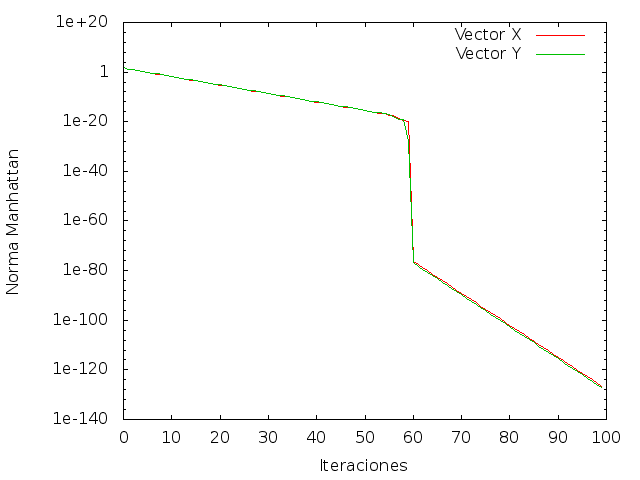
\includegraphics[scale=0.4]{imagenes/hits-movie.png}
    \caption{Movies expanded }
\end{subfigure}
  % \end{center}
% \end{figure}
% \begin{figure}[!htb]
% \begin{center}
\begin{subfigure}{.5\textwidth}
    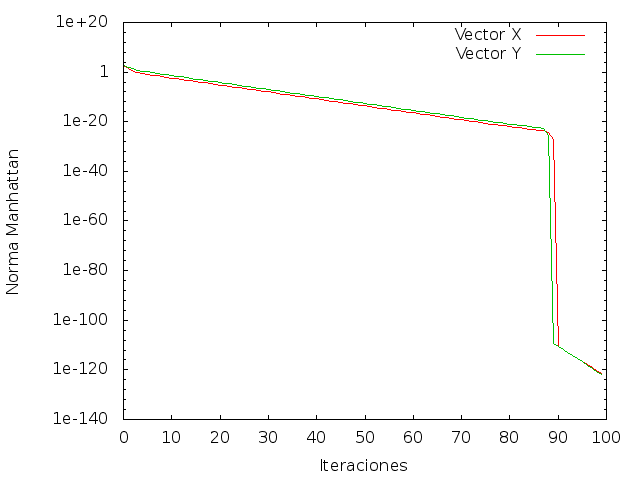
\includegraphics[scale=0.4]{imagenes/hits-stadfor.png}
    \caption{Standford}
\end{subfigure}
    % \end{center}
\end{figure}

En los últimos dos gráficos podemos observar drásticos descensos del valor de la norma cerca de la iteración 60 en el primero y de la 90 en el segundo. Esto es debido a que el valor de la norma es tan bajo que ya no es medible. Por lo tanto consideraremos que justo antes de esos descensos la norma ya convirgió.

\clearpage

\subsection{Tiempos}
Inicialmente hicimos pruebas con dos grafos dados por la cátedra, uno chico y uno grande. Los resultados obtenidos fueron los siguientes:
\begin{itemize}
\item{HITS Abortion(2000 nodos) $=$ 0.694 segundos }
\item{PAGE RANK Abortion(2000 nodos) $=$ 0.104 segundos }
\item{HITS Berkstan(685230 nodos) $=$ 751.63 segundos }
\item{PAGE RANK Berkstan(685230 nodos) $=$ 89.23 segundos }
\end{itemize}

Esto parecería indicarnos que tanto para grafo grandes como chicos, PageRank es más rápido que HITS. Para corroborar esto pensamos en hacer mas pruebas con instancias de distintos tamaños.\\
El siguiente gráfico muestra la evolución del tiempo de computo en función del tamaño de la red para cada algoritmo. La red utilizada en todos los casos es una red estrella en la que todos los nodos (o sitios) apuntan al primero de ellos. Utilizamos este tipo de grafo a modo de ejemplo para tener un caso incial de prueba.
 \begin{figure}[!htb]
 \begin{center}
    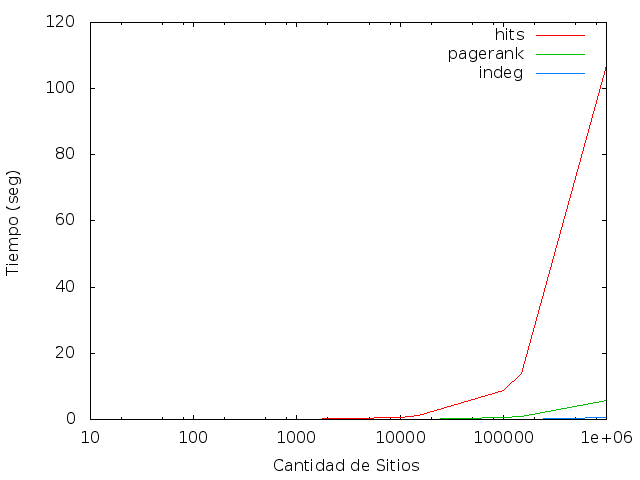
\includegraphics[scale=0.5]{imagenes/Tiempos.png}
    \caption{Tiempo de ejecución en función del tamaño de la red}
    \end{center}
 \end{figure}

Como esto no alcanza para sacar ninguna conjetura debido a que es para un caso particular pensamos en hacer mas pruebas. Lo que provoca que el cálculo sea mas o menos complejo reside en variables desconocidas por nosotros y la cátedra debido a su complejidad. Por lo tanto pensamos en realizar el siguiente test lo mas genérico posible. Para eso hicimos un script (\textit{testTiempos.cpp}) que que va generando grafos aleatoriamente de un tamaño dado y les aplica los 3 algoritmos midiendo sus tiempos de computo.\\ 
\clearpage
Su pseudocógdigo sería:
\begin{algorithm}
\caption{TestGrafosRandom}\label{euclid}
\begin{algorithmic}[1]
\For{$i\ de\ 10\ a\ 11000$}
	\State $\textit{grafo = crearGrafoSinAristas(cantidadNodos=i);}$
	\For{$por\ cada\ nodo\ de\ grafo$}
		\State $\textit{cantidadAristas = random(entre 0 e i);}$
		\For{$j\ de\ 0\ a\ cantidadAristas$}
		\State $\textit{nodo2 = obtenerUnNodoRandom();}$
		\State $\textit{conectar(nodo,nodo2);}$
		\EndFor
	\EndFor	
	\State $\textit{medirTiempo(pageRank(grafo));}$
	\State $\textit{medirTiempo(HITS(grafo));}$
	\State $\textit{medirTiempo(indeg(Grafo));}$
\EndFor
\end{algorithmic}
\end{algorithm}

El resultado obtenido fue el siguiente:
 \begin{figure}[!htb]
 \begin{center}
    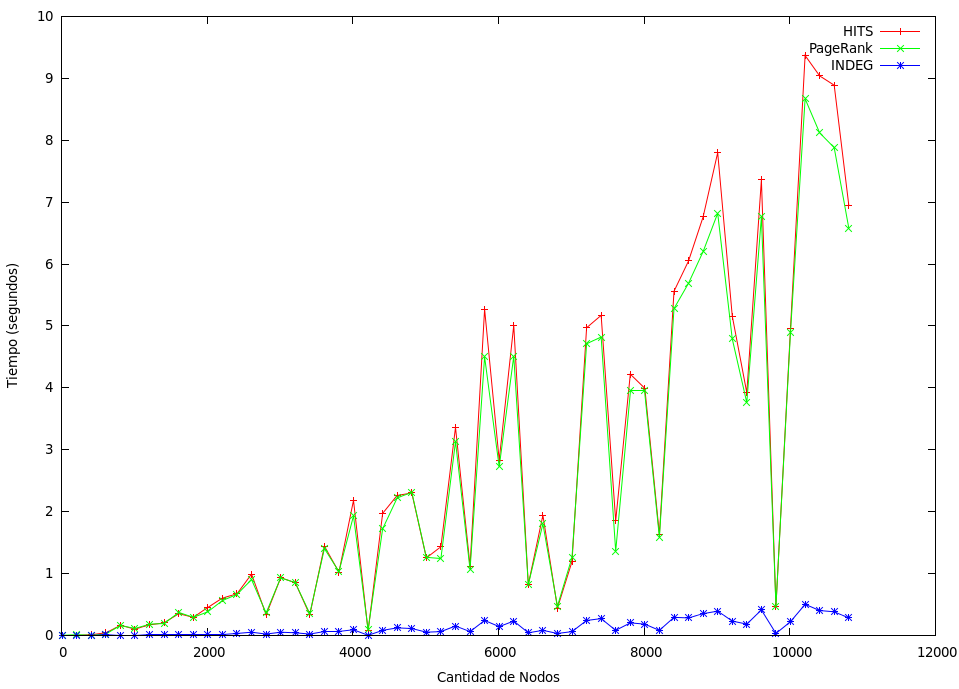
\includegraphics[scale=0.4]{imagenes/grafico_tiempos_sin_filtro.png}
    \caption{Tiempo de ejecución en función de la cantidad de nodos}
    \end{center}
 \end{figure}









